% Particle-decay tree with independent three-point growth at two levels.
\documentclass[border=2pt]{standalone}
\usepackage{tikz}
\usetikzlibrary{trees}

\tikzset{
  particle/.style={draw,circle,minimum size=10mm,inner sep=1pt,fill=cyan!12},
  product/.style={draw,rounded corners=2pt,minimum width=12mm,minimum height=7mm,inner sep=1pt},
  every edge from parent/.style={draw,thick,-stealth}
}

\begin{document}
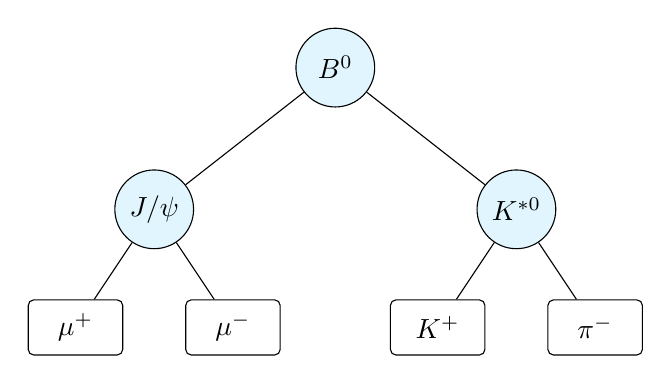
\begin{tikzpicture}[
  level 1/.style={grow via three points={one child at (0,-14mm) and
    two children at (-23mm,-18mm) and (23mm,-18mm)}},
  level 2/.style={grow via three points={one child at (0,-12mm) and
    two children at (-10mm,-15mm) and (10mm,-15mm)}}
]
  \node[particle] {$B^0$}
    child {
      node[particle] {$J/\psi$}
      child {node[product] {$\mu^+$}}
      child {node[product] {$\mu^-$}}
    }
    child {
      node[particle] {$K^{*0}$}
      child {node[product] {$K^+$}}
      child {node[product] {$\pi^-$}}
    };
\end{tikzpicture}
\end{document}
